\section{Evaluation}

\subsection{Results}

\begin{figure}
	\centering
 	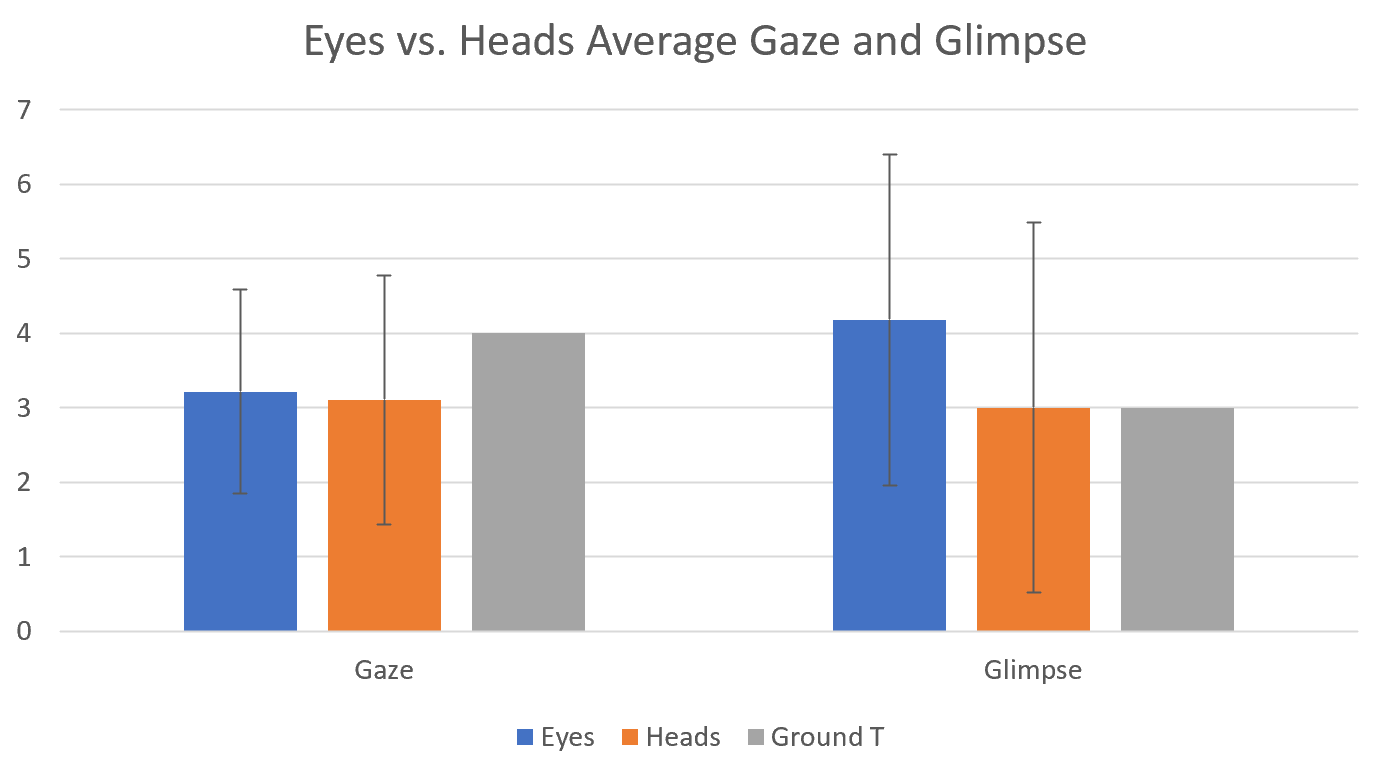
\includegraphics[width=\textwidth]{Result_F1.png}
	\caption{The eye model and head model gaze and glimpse times comparison with ground truth}
	\label{fig:e1-ga}
\end{figure}

In E1 experiment, all participants reported that they had been looked at. But in experiment H2, 14/15 participants reported that they had been looked at. The Figure \ref{fig:e1-ga} shows the gaze and glimpse number in both experiments E1 and H2 . The glimpse result is more sparse with the highest reported number being 9 (For E1), and the lowest being 1.5. This result matches our expectation. 

We did not reveal the questions before the experiments because we think it will cause the participants to pay extra attention to finding the answers, which will corrupt the original experiment purposes. Instead we only asked the participants to observe carefully while performing the experiments. Thus it’s expected that participants could not remember exactly what they just saw when answering those questions. We believe this created some outliers. For example, P11 is the only one who reported he had not been looked at in the H2.

We asked the participants ``Which one attracted your attention more: eyes(0) or heads(100)?" three times during the experiments. ``Watching" is E1 and H2, ``speaking" is after E3 and H3, and ``overall" is in the final question section. Results show that with all the tasks, participants felt their attention was attracted by the head model more than the eye model. Both the eye model and the head model universally make participants notice that they were being looked at. Participants have a sense of being looked with an average of 70.86\% due to the head and 29.14\% due to eyes (i.e. 3D heads make it more obvious to feel the glimpse and gaze), shown in Figure \ref{fig:e1-eye-vs-head}. 

\begin{figure}
	\centering
 	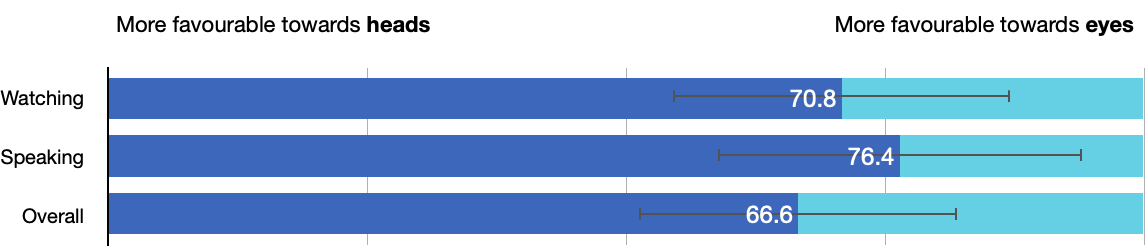
\includegraphics[width=\textwidth]{Result_F4.png}
	\caption{The attention distribution of heads and eyes in watching, speaking and overall tasks}
	\label{fig:e1-eye-vs-head}
\end{figure}

In experiment E3 and experiment H3, participants were asked to rate their nervous level, focus level, and engagement level compared with traditional WVC when using the eye model and the head model. As shown in Figure \ref{fig:e3h3}, 0 indicates our model is 100\% less nervous, focusing and engaging than the traditional WVC. 100 indicates our model is 100\% more nervous, focusing, and engaging than traditional WVC. 50 indicates our model is equivalent with traditional WVC. 

\begin{figure}
	\centering
 	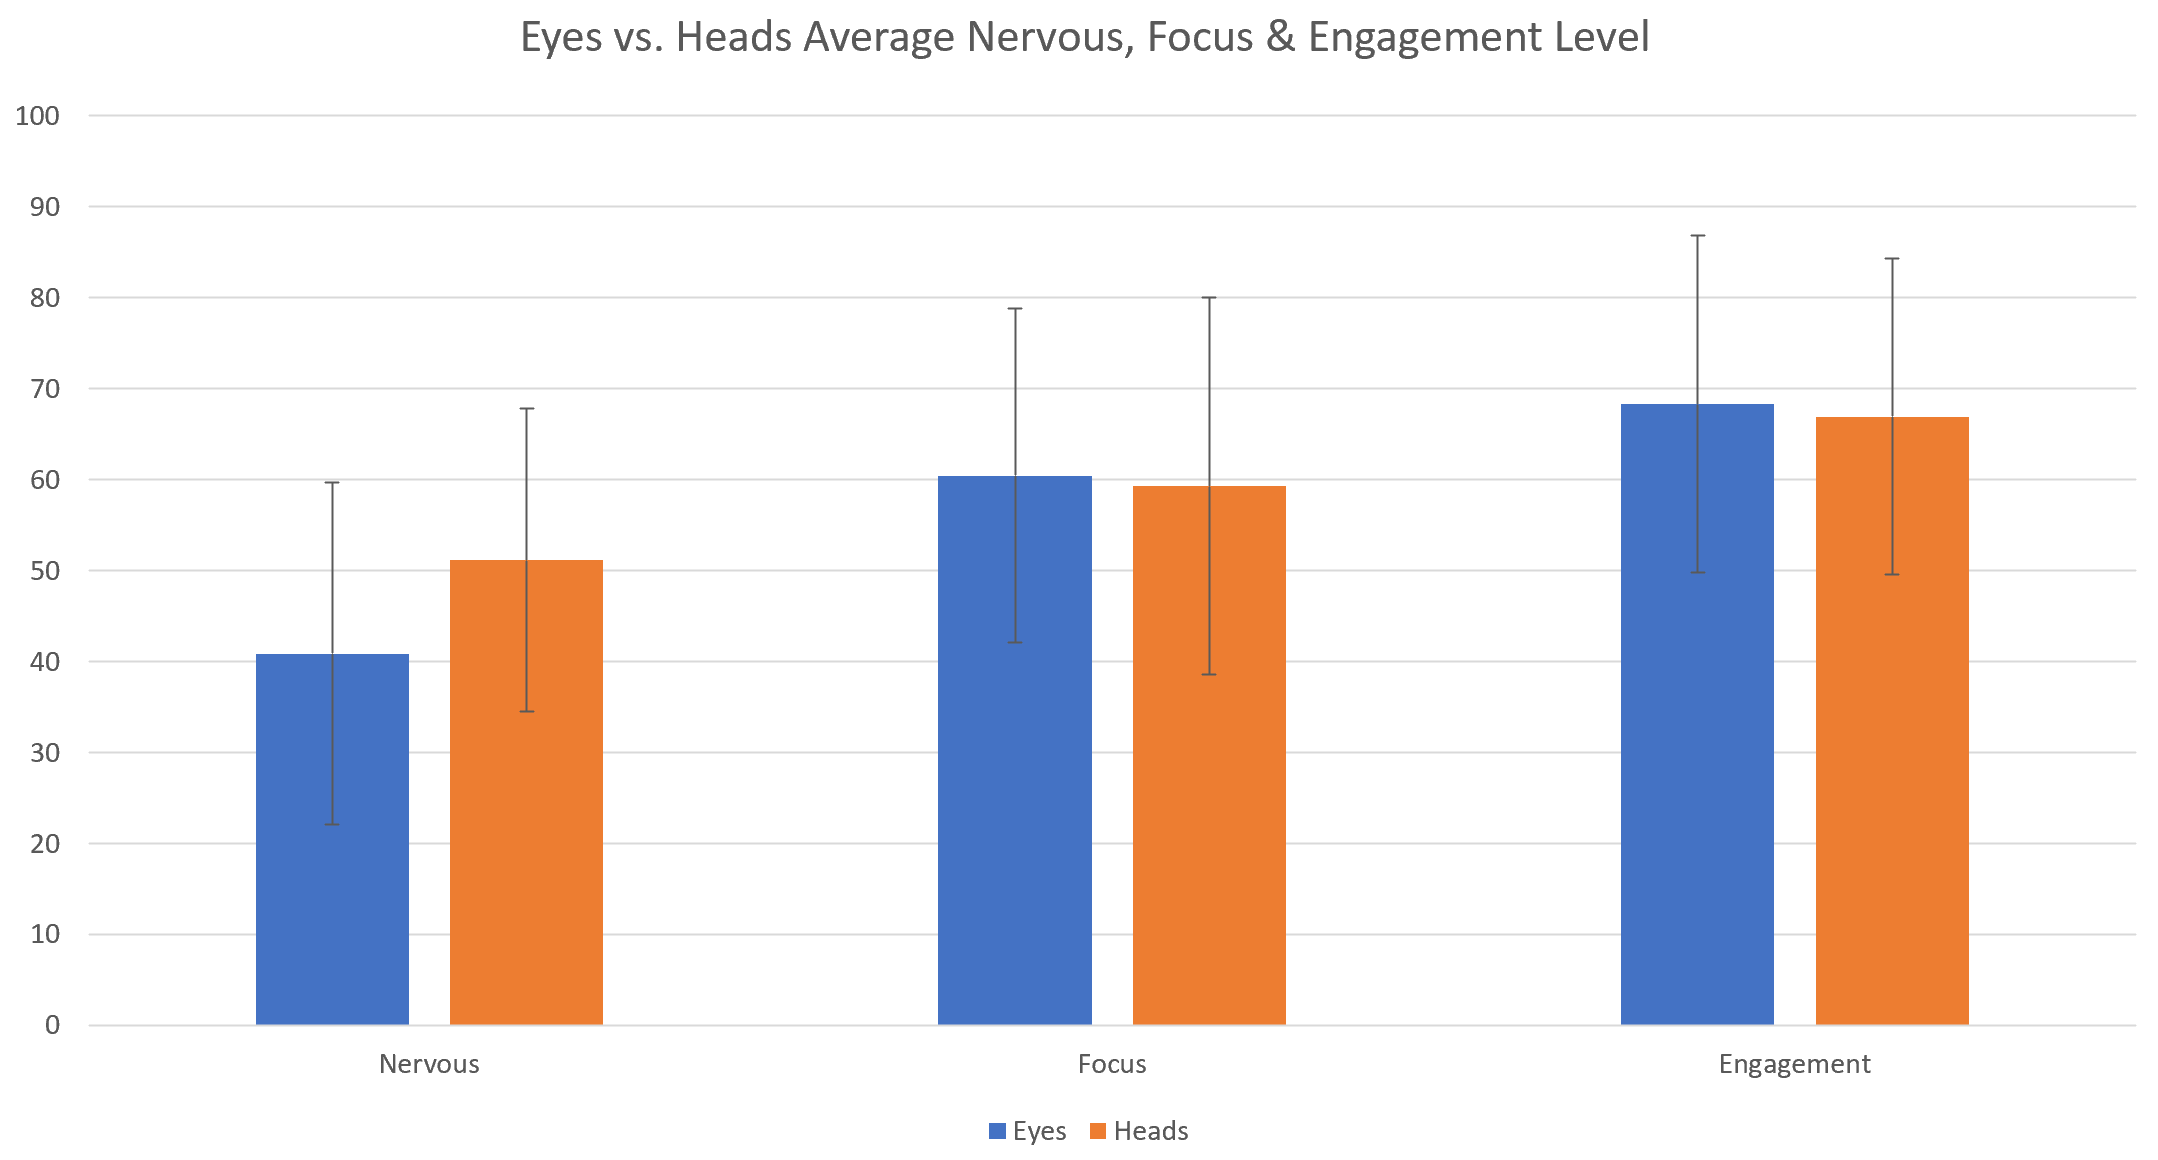
\includegraphics[width=\textwidth]{Result_F3.PNG}
	\caption{Nervousness, focus, and engagement levels reported by the participants as they are asked to speak/present in a room of mock-avatar listeners (E3, H3)}
	\label{fig:e3h3}
\end{figure}

The eye model (E3) average nervous level  is 40.86, and the head model (H3) average nervous level 51.14. This shows that the head model makes participants more nervous than the eye model. The focus level and engagement level for the eye model and the head model does not show significant differences. However, participants reported their focus level and engagement level are enhanced (average focus level is 60.43 for E3, 59.29 for H3; and average engagement level is 68.29 for E3, 66.93 for H3) compared with traditional WVC systems. 


% \textbf{//////////////////////////////////}
% \newline 

The relationship between A,B,C,D were much observed and interpreted clearly (universally) when using heads (H4).
P1, P5, P9, P11, P13 all think compared to the eye model, the head model is much easier to interpret the relationships among other people.
Furthermore, P1 and P5 noted that a few avatars were not participating in the mock-discussion as much.

Unfortunately, while attempting to do quantitative analysis on participant-submitted relationship matrices, we observe that the values in the arrows shown in Figure \ref{fig:relmatrix} were more
closely related to the dynamics in the dialog, rather than eye contact or gaze.

Figure \ref{fig:matrix-mse} shows the mean-squared error (MSE) of the relationship matrix response.
Eventhough users reported having an easier time
seeing using head avatars, they were not any better at correctly perciving the interaction and relationships.
There average increase in misperceptions/errors when switched to heads; and according to user responses,
this could be attributed to head avatars being more distracting.
But it's worth noting that the best-case of MSE decreases when switching from eyes to heads.

Finally, Figure \ref{fig:matrix-attention} shows the magnitude of the user responses between eye avatars and head avatars.
There is a slight increase in percived attention amongst avatars when using heads.
However, this change is very insignificant and could be result of variance/noise.

Generally, the relationship matrix study is not conclusive, and more scenarios and test participants is needed.

\begin{figure}
	\centering
 	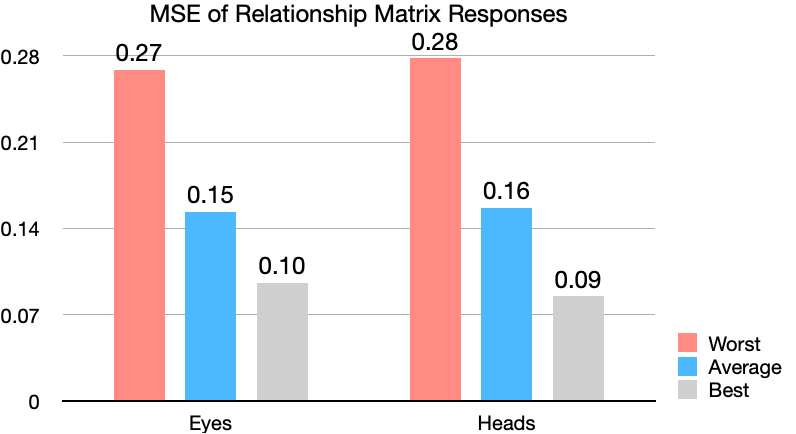
\includegraphics[width=\textwidth]{matrix-mse.png}
	\caption{Mean-squared error of relationship matrix responses (E4, H4)}
	\label{fig:matrix-mse}
\end{figure}

\begin{figure}
	\centering
 	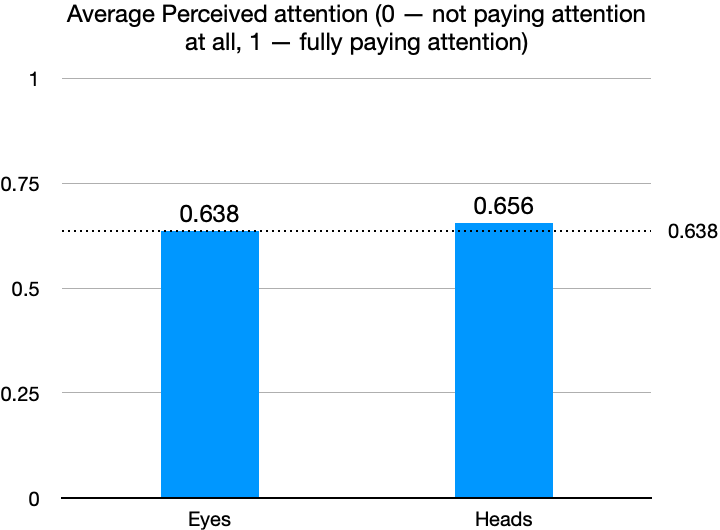
\includegraphics[width=\textwidth]{matrix-amp.png}
	\caption{Normalized mean magnitude of the responses (higher means more percieved attention) (E3, H3)}
	\label{fig:matrix-attention}
\end{figure}

% \textbf{TODO: analysis diagrams (Muchen)}

% \newline
% \textbf{/////////////////////////////////}
% \newline

% \textbf{TODO: Figure 4 Here} \newline



% \begin{figure}
% 	\centering
%  	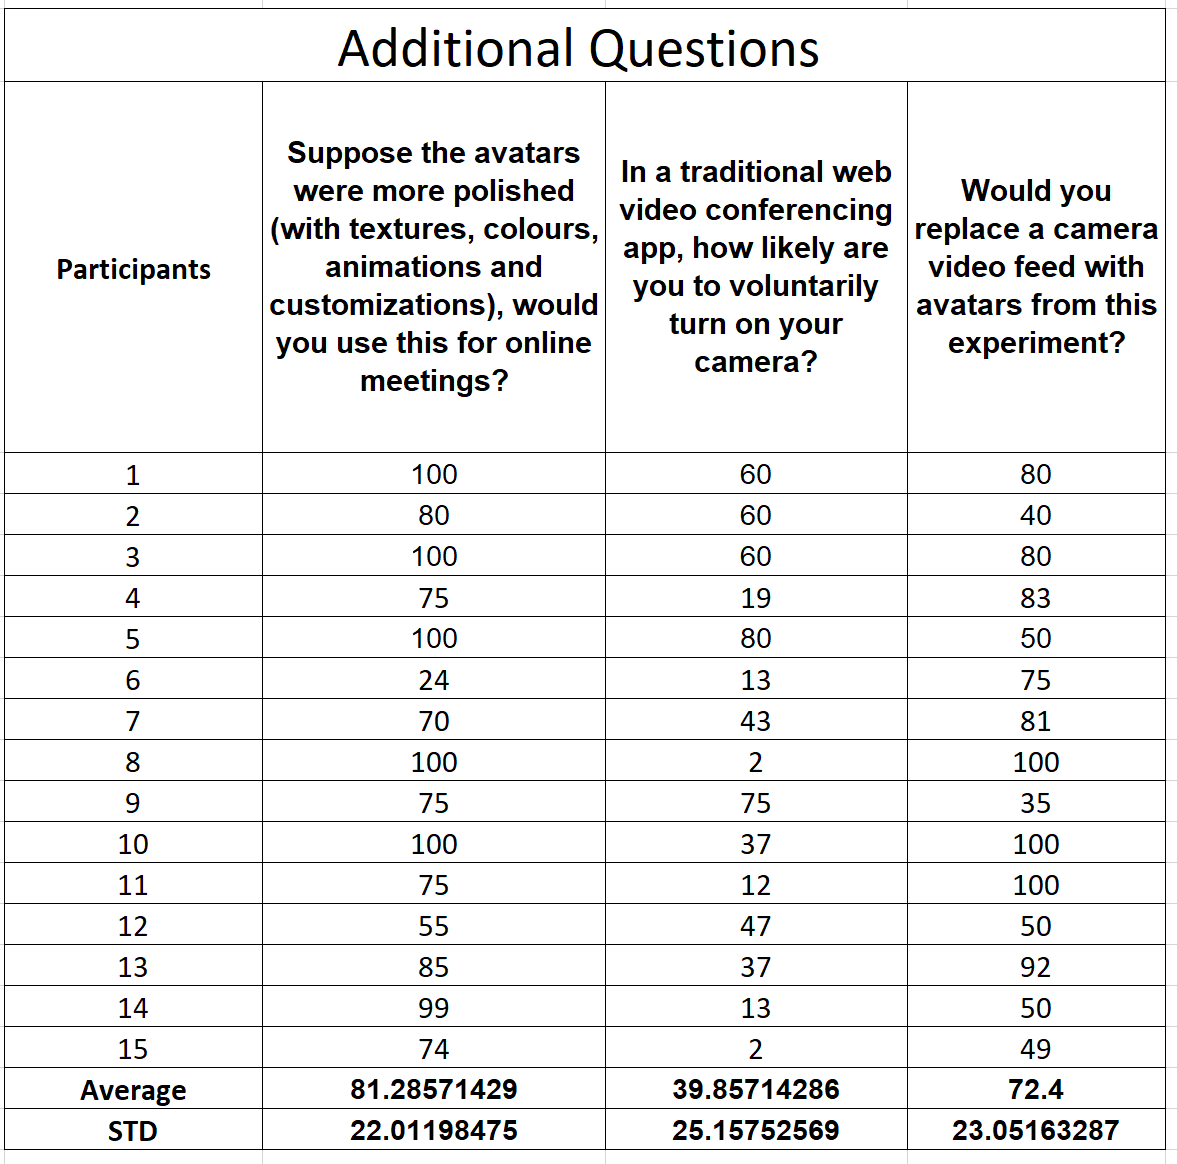
\includegraphics[width=0.45\textwidth]{Result_T1.png}
% 	\caption{The eye model and head model gaze and glimpse times comparison with ground truth}
% 	\label{fig:e1-ga}
% \end{figure}

Participants generally want to use head avatars for online meeting if the avatars were more polished. (Average 81.29 STD 22.01) 
Participants generally would feel comfortable (Average 72.4 STD 23.05) replacing their camera video with the head avatar in certain situations, such as when they don’t want to be distracted by what people are wearing, background, or if themselves don’t want to be seen. 


\section{Discussions}

In general, participants rated the eye model makes them feel less nervous than using traditional WVC systems (average nervous level is 40.86, around 9\% less than neutral). However, comments from participants about nervous level are a bit polarizing. P8 thinks the eye model makes him less nervous since ``\textit{Using cartoon eyes to hide the actual person also makes me less nervous.}" P9 has the opposite opinion about this, ``\textit{Only by showing participants' eyes ... makes me more nervous because you can find out whether people are directly gazing at you anytime.}"
Some participants (P3, P5) also indicated that how nervous they felt depends on how comfortable they are with public speaking. If they’re comfortable talking with a large group of people, neither eyes or heads make a difference in nervous levels. P10 thinks he could not accurately rate his nervous level due to his personal preference of looking away from the screen while talking. It made us to think the possibility of implementing an optional feature to always render the presenter’s view on the audience to help those people who do not have strong public speaking skills to reduce their nervous level. 

Some participants (P3, 5, 9, 10, 15) noted that the head movement in the head model is actually more distracting than the eye model. P10 commented  ``\textit{The movement of the head on the screen may break my train of thought.}" P9 also expressed a similar perspective, ``\textit{Looking at people's heads would make me less focused and nervous because I will pay some attention to them and find out whether they are listening or not.}" Indeed, even when users are giving a talk in real life, they would only perceive the general reactions of the majority of the audiences. They might not notice when only a few audiences start to look around as long as the majority is paying attention. But our system augmented the ``looking around" movement, which made it very obvious when only a few heads start to shift attention despite that the majority are still paying attention. P5 resonated in the same way and felt disappointed when somebody starts to look around.

 

Focus level between eyes and heads are divided: some people (P3, P5) think that the eyes have less focus because it’s hard to tell who is paying attention. On the contrary, P3, 5, 9, 10, 15 think that head is too obvious and the added animation/motion is more distracting. 
P1, 2, 8, 9 commented that head model is more obvious than eye model. 
P3, 5, 9, 10, 15 noted that the head movement is actually more distracting than the eye model.  

Some participants gave comments beyond our questionnaire after they finished the entire experiments. They indicated that in general, they felt more comfortable with the eye model if they are the one talking, but more comfortable with the head model if they are listening. 
They also suggested that for future work, we should also look into combinations of eyes and heads. They also suggested that we could build a model which provides a combination of eyes and heads interchangeably depending on the needs of the users. They could choose to go into head mode when they are listening to a talk and go into eye mode when they are giving a talk.

P7 brought up a point related to privacy, ``\textit{it’s a  pretty interesting app, which helps keep privacy while enabling interaction.}" Privacy is one of the most controversial problems in online meetings during the pandemic period and solutions like virtual background helped to protect the meeting room privacy but not the user's appearance. Using our app, users could choose to not render their camera feed but an avatar head version of themselves. However, in order to achieve this, real time 3D head reconstruction, WVC, and gaze tracking need to be further integrated.
